
%(BEGIN_QUESTION)
% Copyright 2012, Tony R. Kuphaldt, released under the Creative Commons Attribution License (v 1.0)
% This means you may do almost anything with this work of mine, so long as you give me proper credit

Wire a set of ``Start'' and ``Stop'' industrial pushbutton switches to a motor starter unit to form a working start/stop motor control circuit.  The 120 VAC power cord is for control power only -- there will be no three-phase power connected to the contactor's power terminals.  All electrical connections must be made using a terminal strip (no twisted wires, crimp splices, wire nuts, spring clips, or ``alligator'' clips permitted).

$$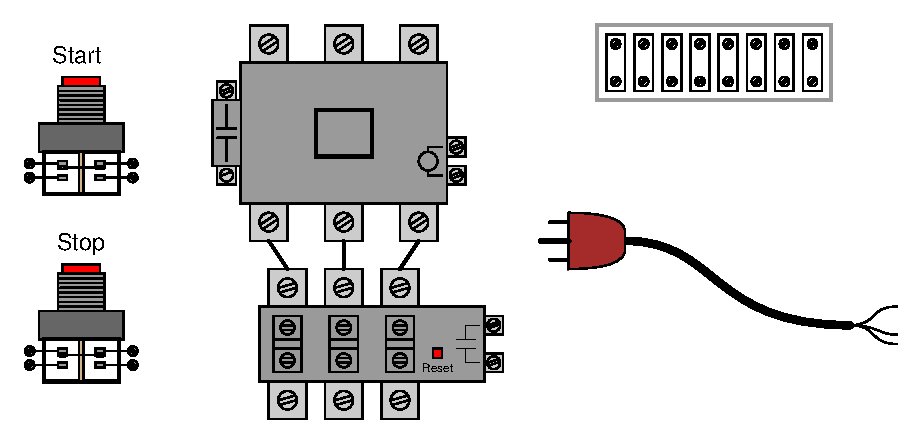
\includegraphics[width=15.5cm]{i01261x01.eps}$$

The following components and materials will be available to you during the exam: {\bf three-phase contactor and overload heater assembly}, complete with auxiliary contacts ; {\bf terminal strips} ; lengths of {\bf hook-up wire} ; assorted {\bf pushbutton switches} ; {\bf 120 VAC power cord} for control power ; {\bf fuse} and {\bf fuseholder}.

\vskip 10pt

You will be expected to supply your own screwdrivers and multimeter for assembling and the circuit.  The instructor must perform a basic inspection of the power wiring before you are allowed to power up the circuit.

\vskip 10pt

Since there will neither be three-phase power nor a three-phase electric motor available, the completed circuit will be able to latch on and off, but will not actually control power to any load.

\vfil 

\underbar{file i01261}
\eject
%(END_QUESTION)





%(BEGIN_ANSWER)

 
%(END_ANSWER)





%(BEGIN_NOTES)


%INDEX% Mastery exam performance exercise (circuit), wire start/stop pushbuttons to a motor starter

%(END_NOTES)


